\chapter{Open Source MANO}
\label{ch:osm}
\section{Configuration requirements}
Open Source MANO (OSM) Release FOUR:
		\begin{itemize}		
	\item MINIMUM: 2 CPUs, 4 GB RAM, 20GB disk and a single interface with internet access
	\item RECOMMENDED: 2 CPUs, 8 GB RAM, 40GB disk and a single interface with internet access
	\item Ubuntu16.04 (64-bit variant required) as base image 
	(\hyperlink{name}{http://releases.ubuntu.com/16.04/})
		\end{itemize}
\section{Open Source Mano Installation}
\subsection{Steps for Installation:}
\begin{itemize}
	\item Downloading latest version of OSM
	\begin{lstlisting} 
wget https://osm-download.etsi.org/ftp/osm-4.0-four/install_osm.sh
	\end{lstlisting}
	
	\item Installing OSM
	\begin{lstlisting} 
chmod +x install_osm.sh
$ ./install_osm.sh 2>&1 | tee osm_install_log.txt
\end{lstlisting}
\end{itemize}
\subsection{Verifying installation from the OSM GUI:}
\begin{itemize}
\item Accessing GUI:\\
Access http://1.2.3.4, replacing 1.2.3.4 with the IP address of your host.\\
Login using Userid : admin , password : admin


\begin{figure} [H]
	\centering
	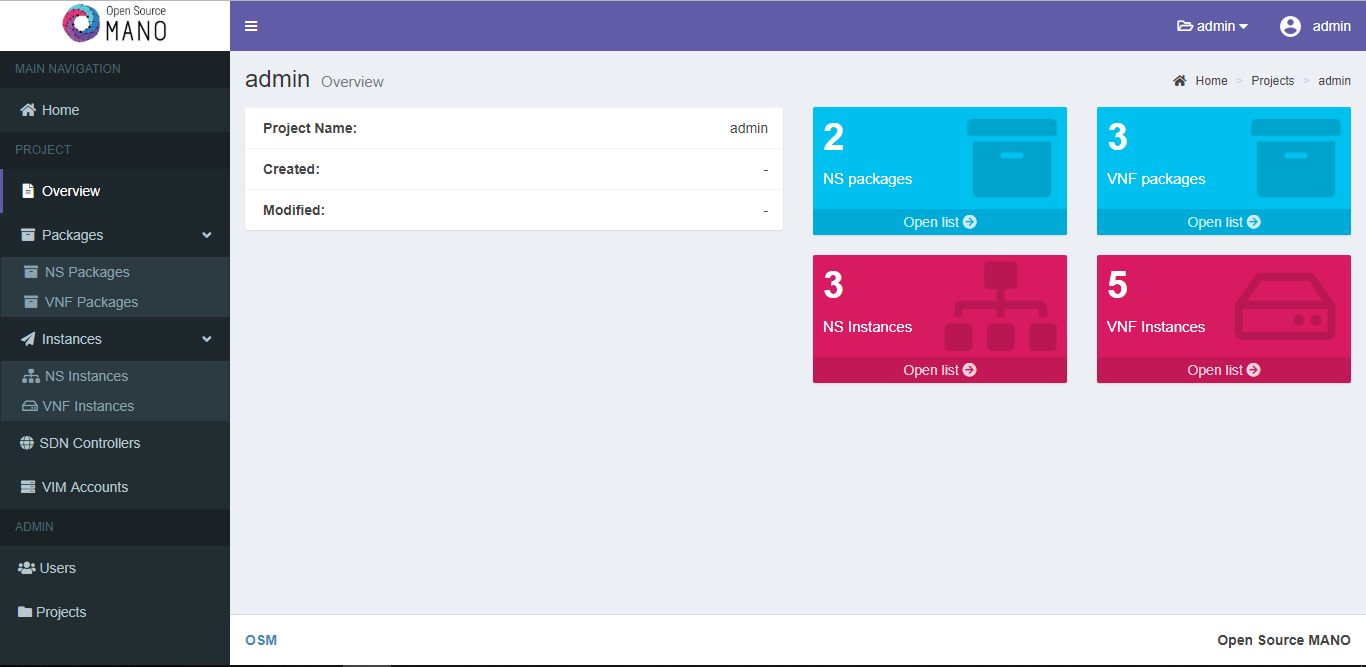
\includegraphics[width=0.6\linewidth]{figures/Sh1}
	\caption{OSM GUI}
\end{figure}

\item Verify 10 docker containers were created:

\begin{lstlisting} 
docker stack ps osm |grep -i running
docker service ls
\end{lstlisting}

\end{itemize}

\section{VIM Installation}

\subsection{Steps to install openstack using devstack are as follows:}

\begin{itemize}
\item Create a user “stack”
\begin{lstlisting}
sudo useradd -s /bin/bash -d /opt/stack -m stack
echo "stack ALL=(ALL) NOPASSWD: ALL" | sudo tee /etc/sudoers.d/stack
sudo su -stack
\end{lstlisting}
\item Clone the devstack repository

\begin{lstlisting}
git clone https://git.openstack.org/openstack-dev/devstack
cd devstack
\end{lstlisting}

\item Create and configure the local.conf file
\begin{lstlisting}
[[local|localrc]]
ADMIN_PASSWORD=password
DATABASE_PASSWORD=$ADMIN_PASSWORD
RABBIT_PASSWORD=$ADMIN_PASSWORD
SERVICE_PASSWORD=$ADMIN_PASSWORD
\end{lstlisting}

\item Execute the command
\begin{lstlisting}
./stack.sh
\end{lstlisting}
\pagebreak
\item After installation check and verify from openstack horizon GUI:
\begin{itemize}
\item Access http://1.2.3.4, replacing 1.2.3.4 with the IP address of your host.
Login using Userid : admin , password : admin
\end{itemize}
\begin{figure} [H]
	\centering
	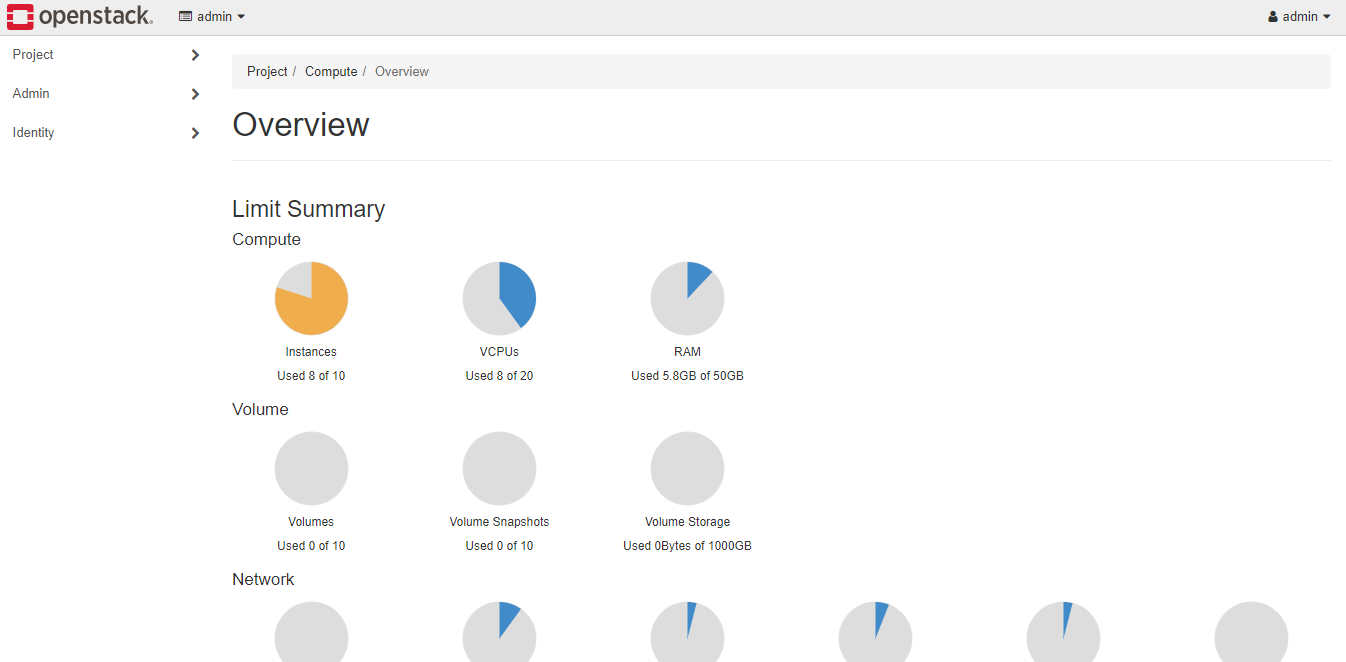
\includegraphics[width=0.5\linewidth]{figures/sh2}
	\caption{Open Stack Dashboard}
\end{figure}
\end{itemize}
\section{Configure openstack for OSM}
\begin{itemize}

\item Verify that Openstack API endpoints are reachable from OSM (particularly from RO container):
\begin{itemize}
\item Login to openstack  API access from the horizon GUI.
\item Click on DOWNLOAD OPENSTACK RC FILE (API version 3).
\item Copy the OS\_AUTH\_URL variable value.
\item Paste in the browser or do a curl from the VM where OSM is installed to check its reachability. 
\end{itemize}

\item Create a management network, with DHCP enabled, reachable from OSM (particularly from VCA container)
\begin{itemize}
\item Login to openstack horizon GUI.
\item Go to admin-> create network.
\item Give the project name as your project ( default:admin)
\item Give a network name -> mgmt.
\item Give a network subnet name and network address (10.208.1.0/24). 
\item Keep the Network Address source as 'ENTER NETWORK ADDRESS MANUALLY'.
\item Keep Gateway IP blank.
\item In Allocation Pools, give the IPs:  start=10.208.0.2,end=10.208.0.254.
\item Leave DNS Name servers and Host Routes blank and click create.
\end{itemize}
\begin{figure}[h]
	\centering
	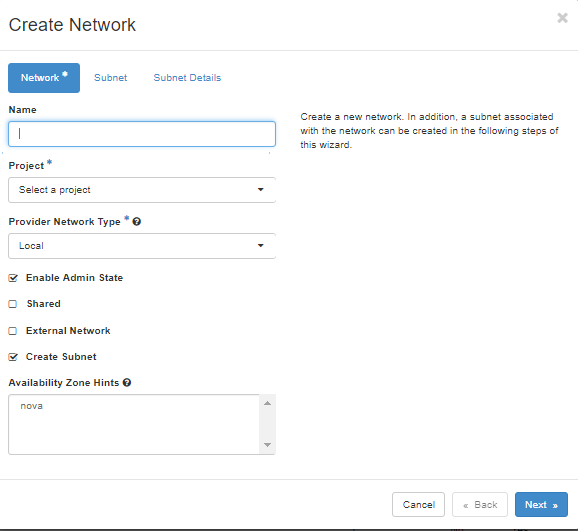
\includegraphics[width=0.4\linewidth]{figures/sh11}
	\caption{Creating a Network in Openstack}
\end{figure} 

\item creating a valid tenant/user
\begin{itemize}
\item Login to openstack horizon gui.
\item Go to identity-> create user.
\item Give the project name as your project ( default:admin)
\item Give a user name -> tenant.
\item Give the role also as admin and click create.
\end{itemize}
\begin{figure}[H]
	\centering
	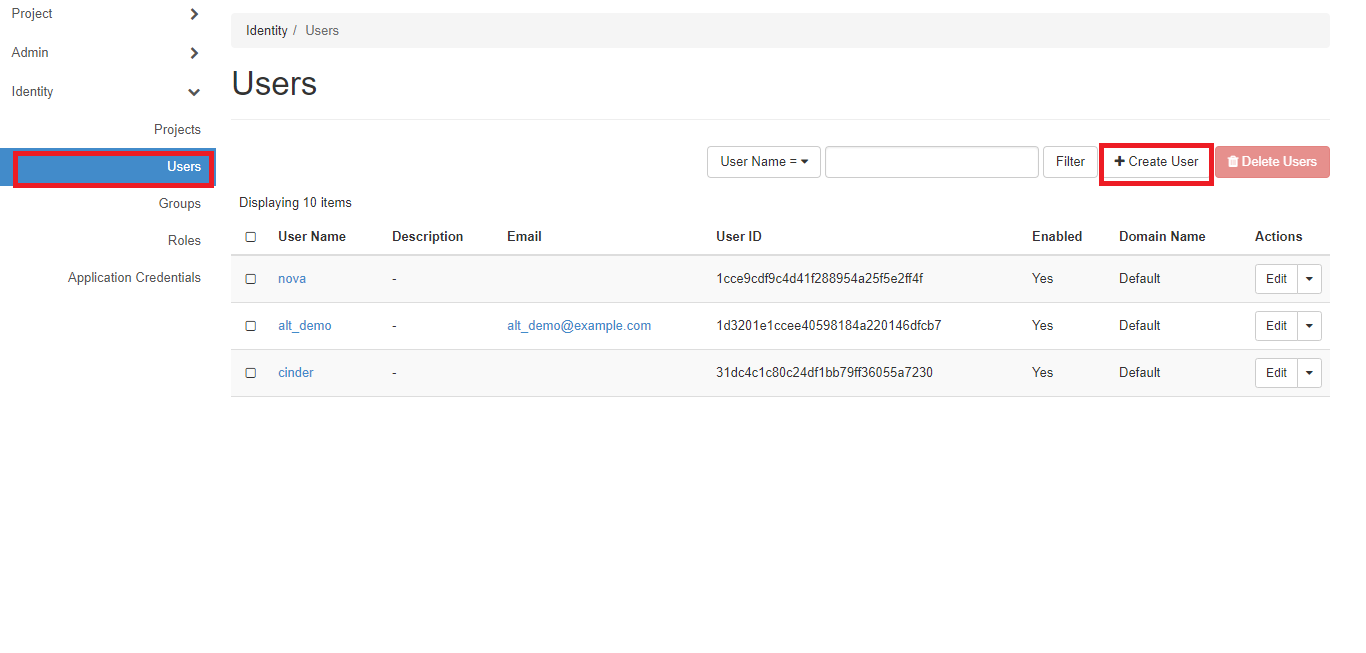
\includegraphics[width=0.5\linewidth]{figures/sh9}
	\caption{creating a valid tenant/user in openstack}
		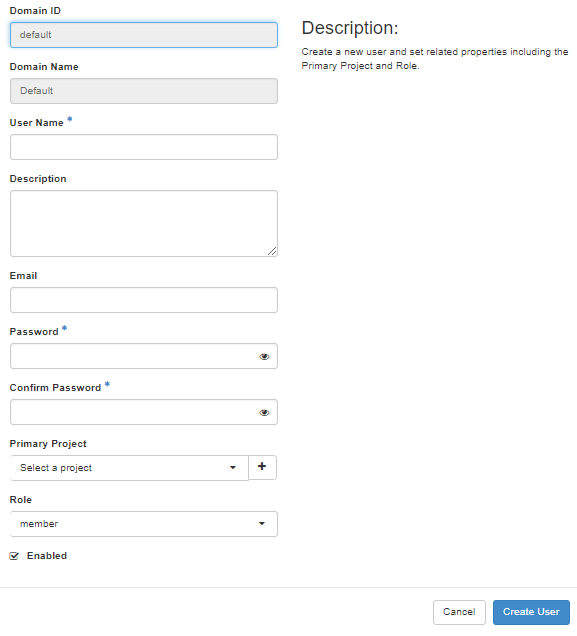
\includegraphics[width=0.5\linewidth]{figures/sh10}
	\caption{creating a valid tenant/user in openstack}
\end{figure}
\pagebreak
\item Uploading VM image(s) to the VIM(s)
\begin{itemize}
\item Download the image from the following link: (\hyperlink{name}{http://download.cirros-cloud.net/0.3.4/cirros-0.3.4-x86\_64-disk.img})
\item Login to openstack horizon gui.
\item Go to admin -> Compute -> Images and click on create image.
\item Give the image name 'cirros034'
\item Upload the downloaded image file in step 1.
\item Choose the image format as QCOW2 : QEMU Emulator
\item Click on create image.
\end{itemize}
\begin{figure} [h]
	\centering
	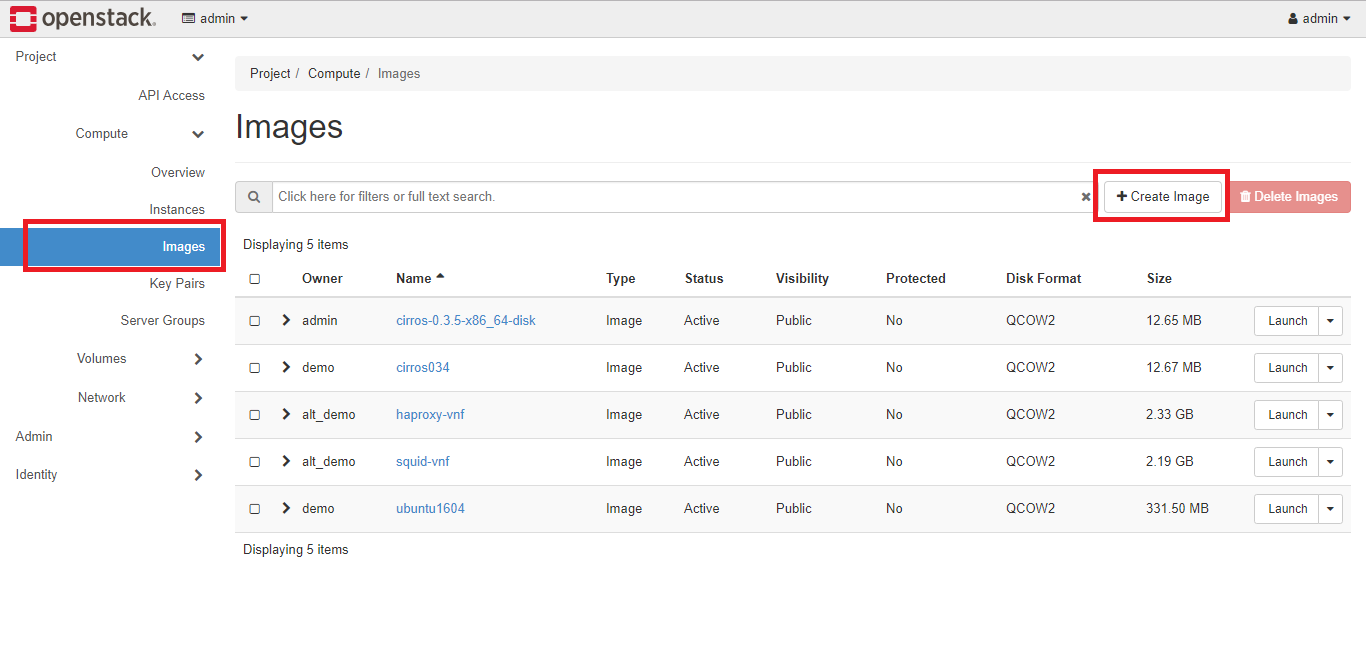
\includegraphics[width=0.5\linewidth]{figures/sh8}
	\caption{Uploading VM image to VIM in openstack}
\end{figure}
\item Adding VIMs to OSM
\begin{itemize}
\item Login to OSM and click on VIM Accounts.
\item Click on new VIM.
\item Give a name to your VIM instance and choose openstack from the type dropdown.Give the VIM URL as the OS\_AUTH\_URL variable value in openstack's rc file.
\item Enter the VIM userid and password as the login userid and password for openstack horizon gui.
\item Give the tenant name as admin/tenant.
\item Click on create.
\end{itemize}
\begin{figure} [h]
	\centering
	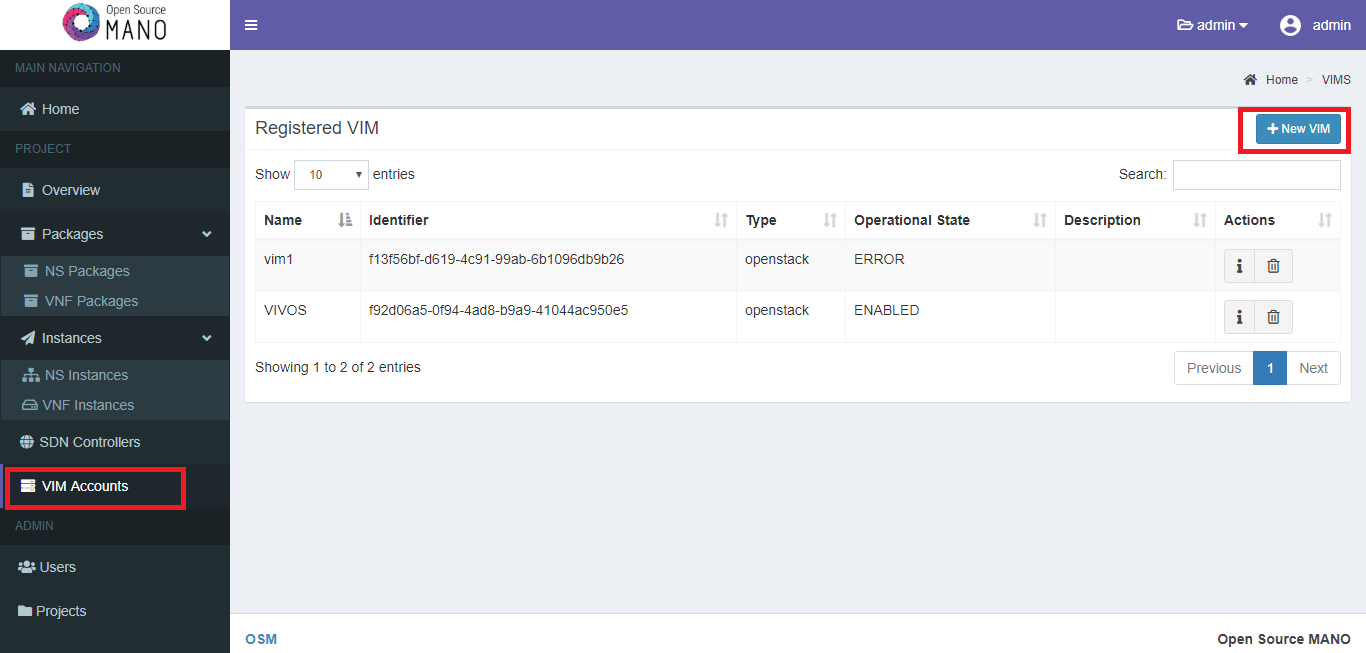
\includegraphics[width=0.5\linewidth]{figures/sh6}
	\caption{Adding VIMs to OSM}
	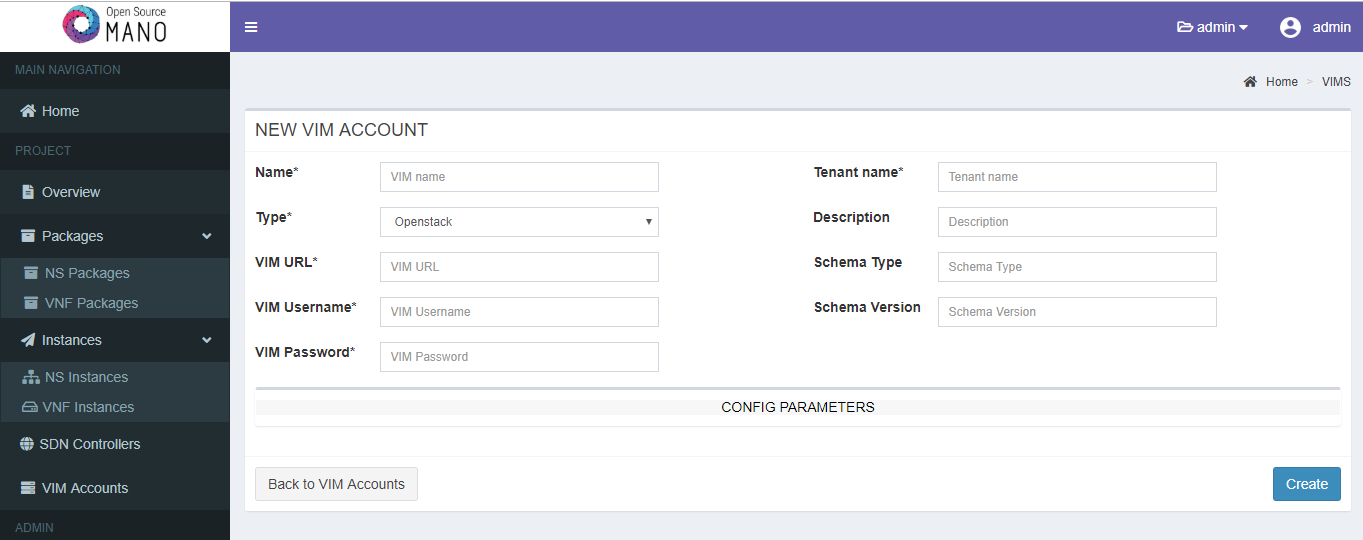
\includegraphics[width=0.5\linewidth]{figures/sh7}
	\caption{Adding VIMs to OSM}
\end{figure}
\end{itemize}
\newpage
\section{Deploying Network Service}
First download the required VNF and NS packages from this URL: \hyperlink{name}{(https://osm-download.etsi.org/ftp/osm-3.0-three/examples/cirros\_2vnf\_ns/)}
\begin{itemize}
\item On-boarding a VNFD
\begin{itemize}
\item From the UI , Go to Projects --> Admin --> VNF Packages (Open List)
\item Click on the Onboard VNFD button
\item Drag and drop the VNF package file cirros\_vnf.tar.gz in the importing area.
\end{itemize}
\begin{figure} [H]
	\centering
	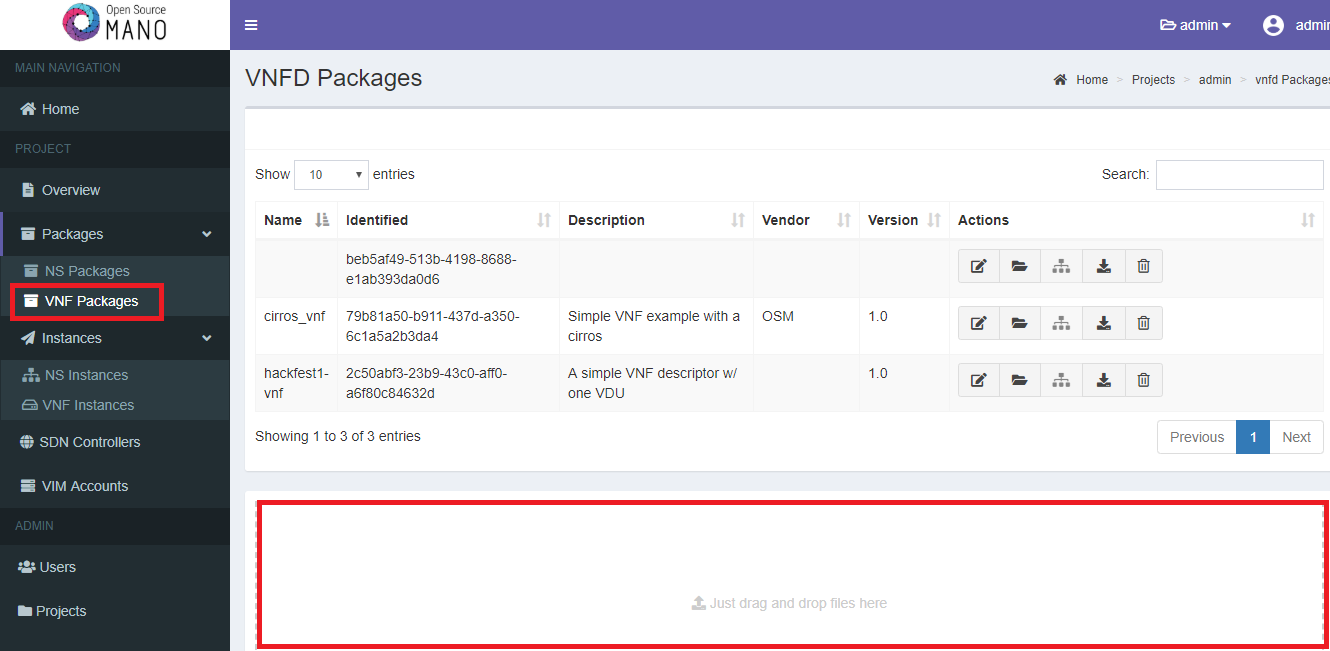
\includegraphics[width=0.5\linewidth]{figures/sh4}
	\caption{On-boarding of VNFD in OSM}
\end{figure}

\item Onboarding a NS
\begin{itemize}
\item From the UI, Go to Projects --> Admin --> NS Packages (Open List)
\item Click on the Onboard NSD button
\item Drag and drop the NS package file cirros\_2vnf\_ns.tar.gz in the importing area.
\end{itemize}
\begin{figure} [H]
	\centering
	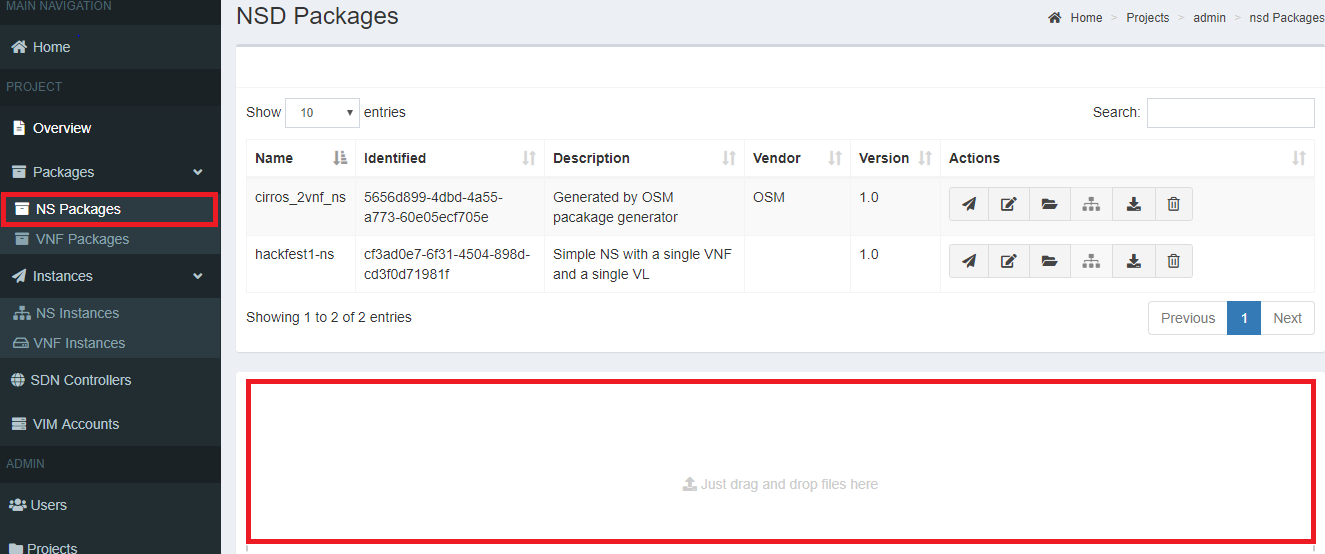
\includegraphics[width=0.5\linewidth]{figures/sh3}
	\caption{On-boarding of NS in OSM}
\end{figure}


\item Instantiating the NS
\begin{itemize}
\item From the UI, Go to Projects --> Admin --> NS Packages (Open List)
\item Next the NS descriptor to be instantiated, click on Launch
\item Fill the form, adding at least a name and selecting the VIM
\end{itemize}
\begin{figure} [H]
	\centering
	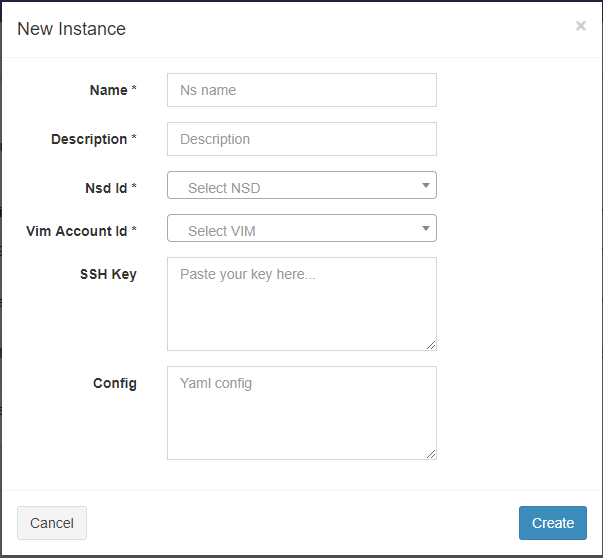
\includegraphics[width=0.5\linewidth]{figures/sh5}
	\caption{Initiating of NS in OSM}
\end{figure}
\end{itemize}
